\documentclass[12pt]{article}
\usepackage[margin=0.8in]{geometry}
\usepackage{amsmath}
\usepackage{hyperref}
\usepackage{graphicx}

\title{Numerical analysis: Assignment 3}
\author{Niccolo Zuppichini}
\begin{document}

\maketitle
\section*{Exercise 1}

By definition a vector $v \neq 0$ is an eigenvector if for $\any \lambda$: \\

\begin{equation}
	\label{def:eig}
	A v = \lambda v
\end{equation}

By rearranging \ref{def:eig}: \\

$$A v - \lambda v = (\lambda I - A)v = 0 $$

Because $v \neq 0 $ it holds only if $\textrm{det}(A - \lambda I)$. Therefore \\

\begin{equation}
	\label{calc1}
	\textrm{det}(A - \lambda I) \implies (\lambda - a) (\lambda - c) - b^2 = 0
\end{equation}

Solving \ref{calc1}: \\


$$(\lambda - a) (\lambda - c) - b^2 = ac - c \lambda - a \lambda +\lambda^2 -b^2 = $$
$$ \lambda^2 - (a+c) \lambda +ac - b^2$$ \\

Then solving the quadratic equation for $\lambda$ yields: \\

$$ \lambda_{1,2} = \frac{(a+c) \pm \sqrt{(a+c)^2 -4ac + 4b^2}}{2} = $$ 
$$ \frac{(a+c) \pm \sqrt{a^2 + c^2 +2ac -4ac + 4b^2}}{2} = $$
$$ \frac{(a+c) \pm \sqrt{a^2 + c^2 -2ac + 4b^2}}{2} = $$
$$ \frac{(a+c) \pm \sqrt{(a-c)^2+ 4b^2}}{2} $$

Then the eigenvalues of $A$ are given by: \\

\begin{align*}\label{eigenvalues}
\lambda_1 = \frac{(a+c) + \sqrt{(a-c)^2+ 4b^2}}{2} \\
\lambda_2 = \frac{(a+c) - \sqrt{(a-c)^2+ 4b^2}}{2} \\
\end{align*}

By recalling the definition of eigenvector \ref{def:eig}, we can find the eigenvectors $v_{1,2}$ by solving:  \\
\begin{equation}
	\label{eq:eig}
	(\lambda_{1,2} I - A)v = 0 
\end{equation}

$$\lambda_{1,2} I - A = 
\begin{bmatrix}
	\lambda_{1,2} -a & b \\
	b & \lambda_{1,2} - c \\
\end{bmatrix}
$$

Solving \ref{eq:eig} leads to: \\

$$ 
\begin{bmatrix}
	\lambda_{1,2} - a & b \\
	b & \lambda_{1,2} - c\\
\end{bmatrix}
\begin{bmatrix}
	x \\
	y \\ 
\end{bmatrix}
= 
\begin{bmatrix}
(\lambda_{1,2} - a) x + b y \\
(\lambda_{1,2} - c) y + b x
\end{bmatrix}
=
\begin{bmatrix}
	0 \\ 0
\end{bmatrix}
$$

Then $(\lambda_{1,2} - c) y + b x \implies x = \frac{(\lambda_{1,2} - c)}{b} y$ and the eigenvectors $v_{1,2}$ are: \\

\begin{align*}
	v_1 = \begin{bmatrix}
		\lambda_{1} - c \\ b
	\end{bmatrix}	 \\
	v_2 = \begin{bmatrix}
		\lambda_{2} - c \\ b
	\end{bmatrix}	 \\
\end{align*}

respectively for eigenvalues $\lambda_{1,2}$. \\

\section*{Exercise 2}

The code can be found in \textit{main.m}. There's not much to comment on the code. I've followed step by step the lecture notes by Prof. Hormann. \\ 

Please note that the code should be in the same directory with the a folder \textit{data} containing the given data for this exercise. \\

\textbf{My results:} \\

$$R = 
\begin{bmatrix}
	  0.3607 &  -0.9327 \\
    0.9327  &  0.3607 \\
\end{bmatrix}
\quad
t = \begin{bmatrix}
	 -1.8213 & 
   -1.5111 \\
\end{bmatrix}
$$
\\

Then the \textit{new points} (i.e. the fitted points) are given by $P_{new} = R*Q + t$

\begin{figure}[h]
\centering
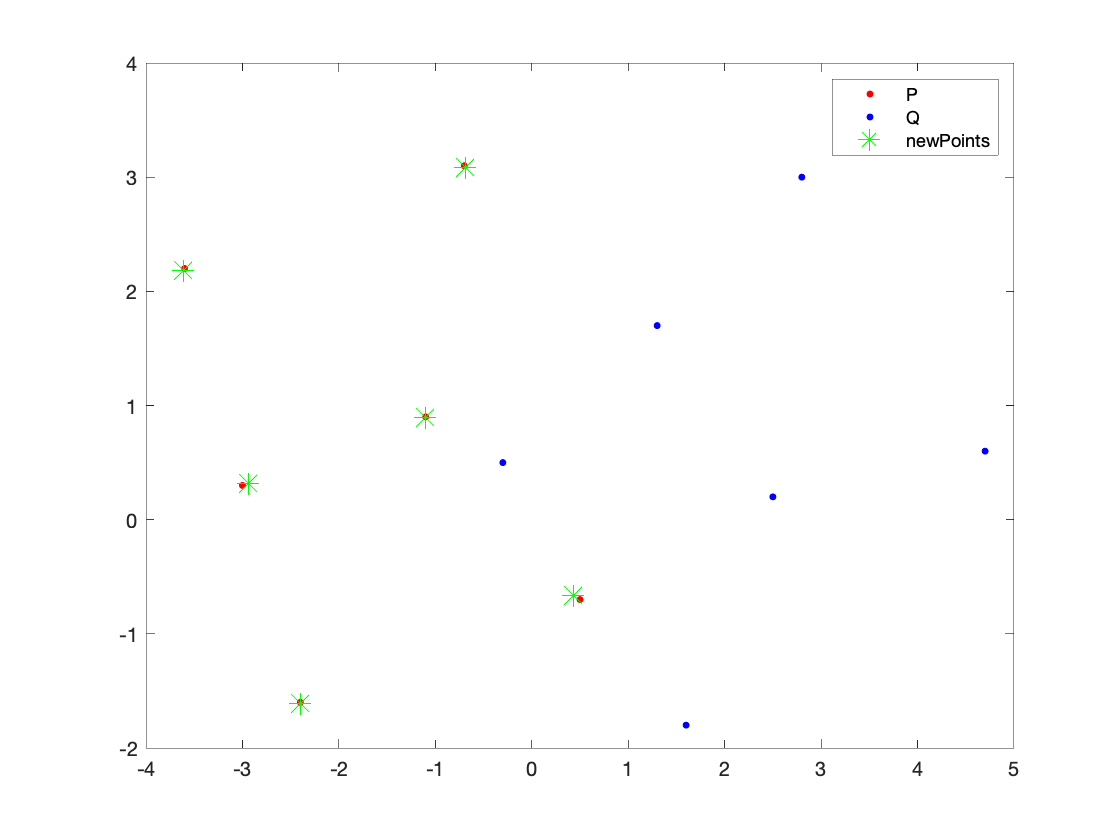
\includegraphics[width=0.95\textwidth]{ex2_result}
\caption{The resulting points after applying the computed rotation and translation}
\label{fig:ex2}
\end{figure}

As figure \ref{fig:ex2} shows, the new points $P_{new}$ are really close to $P$. The $L_{inf}$ norm between $P_{new} - P$ is $0.1610$, which is in my opinion low. The value of $f(R, t)$ is $0.0095$\\

\end{document}